\documentclass[11pt, a4paper, landscape]{article}
\usepackage[utf8]{inputenc}
\usepackage{geometry}
\geometry{a4paper, margin=0.5in, landscape}
\usepackage{tikz}
\usetikzlibrary{shapes, arrows.meta, positioning, calc, matrix}
\usepackage{pgfgantt}
\usepackage{xcolor}
\usepackage{graphicx}

\title{\textbf{EVNet Sentinel: Project Planning}\\ \vspace{0.5cm} Network Diagram, Critical Path, and Gantt Chart}
\author{Group 1}
\date{\today}

\newcommand{\pert}[7]{
  \begin{tabular}{|@{}c@{}|@{}c@{}|@{}c@{}|}
  \hline
  \makebox[0.8cm]{\scriptsize #1} & \makebox[0.9cm]{\scriptsize\textbf{#2}} & \makebox[0.8cm]{\scriptsize #3} \\ \hline
  \multicolumn{3}{|c|}{\parbox{2.5cm}{\vspace{0.15cm}\centering\scriptsize #4\vspace{0.15cm}}} \\ \hline
  \makebox[0.8cm]{\scriptsize #5} & \makebox[0.9cm]{\scriptsize #6} & \makebox[0.8cm]{\scriptsize #7} \\ \hline
  \end{tabular}
}

\begin{document}

\maketitle
\newpage

\section*{1. Project Task Details}
To establish the critical path and network diagrams efficiently, task durations have been logically estimated based on the EVNet Sentinel SRS and DFD.

\vspace{0.5cm}
\begin{center}
\begin{tabular}{|c|l|c|c|}
\hline
\textbf{ID} & \textbf{Task Name} & \textbf{Duration (Days)} & \textbf{Predecessors} \\ \hline
A & Load Datasets & 3 & - \\ \hline
B & Parse \& Scale & 5 & A \\ \hline
C & Mask PII \& Feature Eng & 6 & B \\ \hline
D & Static Models & 12 & C \\ \hline
E & Online Adaptive Model & 15 & C \\ \hline
F & Train \& Tune & 8 & D, E \\ \hline
G & Classification Reports & 5 & F \\ \hline
H & Traffic Simulator & 8 & C \\ \hline
I & Synthetic Injector & 7 & H \\ \hline
J & FastAPI Backend & 10 & G, I \\ \hline
K & Dashboard UI \& Metrics & 10 & J \\ \hline
L & Live Alerts \& Matrices & 8 & K \\ \hline
M & Simulation Controls & 7 & K \\ \hline
N & Anomaly Investigation & 7 & K \\ \hline
O & E2E Integration & 12 & L, M, N \\ \hline
P & Final Evaluation & 6 & O \\ \hline
\end{tabular}
\end{center}

\newpage
\section*{2. Network Diagram and Critical Path}
The highlighted red path indicates the Critical Path: \textbf{A $\rightarrow$ B $\rightarrow$ C $\rightarrow$ E $\rightarrow$ F $\rightarrow$ G $\rightarrow$ J $\rightarrow$ K $\rightarrow$ L $\rightarrow$ O $\rightarrow$ P} (Total: 88 Days $\approx$ 4 Months).\\
Each node follows the standard PERT format:
\begin{center}
\begin{tabular}{|c|c|c|}
\hline
Early Start (ES) & Task ID & Early Finish (EF) \\ \hline
\multicolumn{3}{|c|}{Task Name} \\ \hline
Latest Start (LS) & Duration & Latest Finish (LF) \\ \hline
\end{tabular}
\end{center}

\vspace{0.5cm}
\begin{center}
\resizebox{\textwidth}{!}{
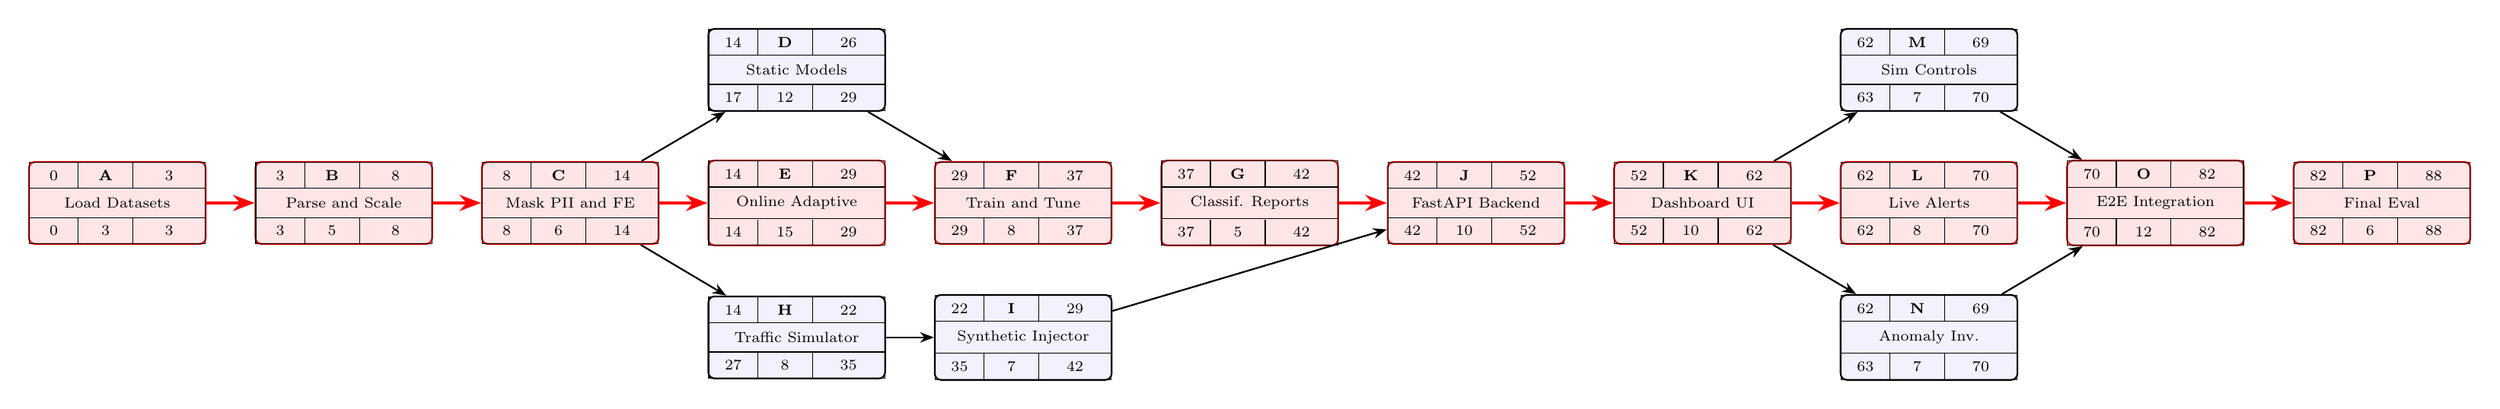
\begin{tikzpicture}[
    task/.style = {rectangle, draw=black, thick, fill=blue!5, inner sep=0pt, rounded corners=3pt},
    critical/.style = {rectangle, draw=red, thick, fill=red!10, inner sep=0pt, rounded corners=3pt},
    arrow/.style = {->, >=Stealth, thick},
    carrow/.style = {->, >=Stealth, ultra thick, red}
]

\matrix [column sep=0.8cm, row sep=0.8cm, ampersand replacement=\&] {
% Row 1
\& \& \& \node[task] (D) {\pert{14}{D}{26}{Static Models}{17}{12}{29}}; \& \& \& \& \& \node[task] (M) {\pert{62}{M}{69}{Sim Controls}{63}{7}{70}}; \& \& \\
% Row 2
\node[critical] (A) {\pert{0}{A}{3}{Load Datasets}{0}{3}{3}}; \& 
\node[critical] (B) {\pert{3}{B}{8}{Parse and Scale}{3}{5}{8}}; \& 
\node[critical] (C) {\pert{8}{C}{14}{Mask PII and FE}{8}{6}{14}}; \& 
\node[critical] (E) {\pert{14}{E}{29}{Online Adaptive}{14}{15}{29}}; \& 
\node[critical] (F) {\pert{29}{F}{37}{Train and Tune}{29}{8}{37}}; \& 
\node[critical] (G) {\pert{37}{G}{42}{Classif. Reports}{37}{5}{42}}; \& 
\node[critical] (J) {\pert{42}{J}{52}{FastAPI Backend}{42}{10}{52}}; \& 
\node[critical] (K) {\pert{52}{K}{62}{Dashboard UI}{52}{10}{62}}; \& 
\node[critical] (L) {\pert{62}{L}{70}{Live Alerts}{62}{8}{70}}; \& 
\node[critical] (O) {\pert{70}{O}{82}{E2E Integration}{70}{12}{82}}; \& 
\node[critical] (P) {\pert{82}{P}{88}{Final Eval}{82}{6}{88}}; \\
% Row 3
\& \& \& \node[task] (H) {\pert{14}{H}{22}{Traffic Simulator}{27}{8}{35}}; \& 
\node[task] (I) {\pert{22}{I}{29}{Synthetic Injector}{35}{7}{42}}; \& \& \& \& 
\node[task] (N) {\pert{62}{N}{69}{Anomaly Inv.}{63}{7}{70}}; \& \& \\
};

% Edges
\draw[carrow] (A) -- (B);
\draw[carrow] (B) -- (C);

\draw[arrow] (C) -- (D);
\draw[carrow] (C) -- (E);
\draw[arrow] (C) -- (H);

\draw[arrow] (D) -- (F);
\draw[carrow] (E) -- (F);
\draw[arrow] (H) -- (I);

\draw[carrow] (F) -- (G);

\draw[carrow] (G) -- (J);
\draw[arrow] (I) -- (J);

\draw[carrow] (J) -- (K);

\draw[arrow] (K) -- (M);
\draw[carrow] (K) -- (L);
\draw[arrow] (K) -- (N);

\draw[arrow] (M) -- (O);
\draw[carrow] (L) -- (O);
\draw[arrow] (N) -- (O);

\draw[carrow] (O) -- (P);

\end{tikzpicture}
}
\end{center}

\newpage
\section*{3. Gantt Chart}

\begin{center}
\resizebox{\textwidth}{!}{
\begin{ganttchart}[
    vgrid,
    hgrid,
    x unit=0.26cm,
    y unit title=0.6cm,
    y unit chart=0.6cm,
    bar/.style={fill=blue!50},
    bar label font=\footnotesize,
    group label font=\bfseries\footnotesize,
    title label font=\footnotesize,
    milestone label font=\itshape\footnotesize
]{1}{88}
\gantttitle{EVNet Sentinel Project Schedule (Days) --- Semester: $\approx$ 4 Months}{88} \\
\gantttitlelist{1,...,88}{1} \\

% Phase 1: Data Preparation (Days 1--14)
\ganttgroup{Phase 1: Data}{1}{14} \\
\ganttbar{A: Load Datasets}{1}{3} \\
\ganttbar{B: Parse \& Scale}{4}{8} \\
\ganttbar{C: Mask PII \& FE}{9}{14} \\

% Phase 2: ML Engine (Days 15--42)
\ganttgroup{Phase 2: ML Engine}{15}{42} \\
\ganttbar{D: Static Models}{15}{26} \\
\ganttbar[bar/.style={fill=red!60}]{E: Online Adaptive Model}{15}{29} \\
\ganttbar{F: Train \& Tune}{30}{37} \\
\ganttbar{G: Classification Reports}{38}{42} \\

% Phase 3: Simulation \& API (Days 15--52)
\ganttgroup{Phase 3: Sim \& API}{15}{52} \\
\ganttbar{H: Traffic Simulator}{15}{22} \\
\ganttbar{I: Synthetic Injector}{23}{29} \\
\ganttbar{J: FastAPI Backend}{43}{52} \\

% Phase 4: Dashboard (Days 53--70)
\ganttgroup{Phase 4: Dashboard}{53}{70} \\
\ganttbar{K: Dashboard UI}{53}{62} \\
\ganttbar[bar/.style={fill=red!60}]{L: Live Alerts}{63}{70} \\
\ganttbar{M: Sim Controls}{63}{69} \\
\ganttbar{N: Anomaly Inv.}{63}{69} \\

% Phase 5: Integration \& Evaluation (Days 71--88)
\ganttgroup{Phase 5: Integration}{71}{88} \\
\ganttbar{O: E2E Integration}{71}{82} \\
\ganttbar{P: Final Eval}{83}{88}

% Links
\ganttlink{elem1}{elem2}
\ganttlink{elem2}{elem3}

\ganttlink{elem3}{elem5}
\ganttlink{elem3}{elem6}
\ganttlink{elem5}{elem7}
\ganttlink{elem6}{elem7}
\ganttlink{elem7}{elem8}

\ganttlink{elem3}{elem10}
\ganttlink{elem10}{elem11}

\ganttlink{elem8}{elem12}
\ganttlink{elem11}{elem12}

\ganttlink{elem12}{elem14}
\ganttlink{elem14}{elem15}
\ganttlink{elem14}{elem16}
\ganttlink{elem14}{elem17}

\ganttlink{elem15}{elem19}
\ganttlink{elem16}{elem19}
\ganttlink{elem17}{elem19}

\ganttlink{elem19}{elem20}

\end{ganttchart}
}
\end{center}

\end{document}
